% !TEX encoding = UTF-8 Unicode
% !TEX TS-program = xelatex
\begin{QUESTIONS}
    \begin{QUESTION}
        \begin{ExamInfo}{101}{學測}{單選}{1}
        \end{ExamInfo}
        \begin{ExamAnsRateInfo}{77}{98}{89}{44}
        \end{ExamAnsRateInfo}
        \begin{QBODY}
            $\sqrt{\frac{1}{5^2}+\frac{1}{4^2}+1}$ 等於下列哪一個選項? 
			\begin{QOPS} 
				\QOP 1.01 
				\QOP 1.05 
				\QOP 1.1 
				\QOP 1.15 
				\QOP 1.21
			\end{QOPS}
        \end{QBODY}
        \begin{QFROMS}
        \end{QFROMS}
        \begin{QTAGS}\QTAG{B1C1-1數與數線}\QTAG{B1C1數與式}\end{QTAGS}
        \begin{QANS}
            (2)
        \end{QANS}
        \begin{QSOLLIST}
        \end{QSOLLIST}
        \begin{QEMPTYSPACE}
        \end{QEMPTYSPACE}
    \end{QUESTION}
    \begin{QUESTION}
        \begin{ExamInfo}{101}{學測}{單選}{2}
        \end{ExamInfo}
        \begin{ExamAnsRateInfo}{87}{99}{98}{64}
        \end{ExamAnsRateInfo}
        \begin{QBODY}
            將邊長為 1 公分的正立方體堆疊成一階梯形立體,如下圖所示,其中第 1 層(最下層)有 10 塊,第 2 層有 9 塊,$\cdots$ ,依此類推。當堆疊完 10 層時,該階梯形立體的表面積(即該立體的 前、後、上、下、左、右各表面的面積總和)為多少?
			\begin{QOPS}
				\QOP 75 平方公分 
				\QOP 90 平方公分 
				\QOP 110平方公分 
				\QOP 130平方公分 
				\QOP 150平方公分
			\end{QOPS}
			
			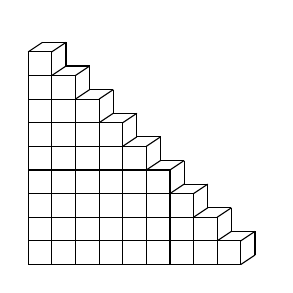
\begin{tikzpicture}[scale=.3]
				\begin{scope}
						\draw (0,0) to (9,0);
						\draw (0,0) to (0,9);
						\foreach \i in {1,2,3,...,9}{
								\draw (0,\i) to (10-\i,\i);
								\draw (\i,0) to (\i,10-\i);
								\draw (\i-1,10-\i) to (\i-.4,10.4-\i);
								\draw (\i,10-\i) to (\i+.6,10.4-\i);
								\draw (\i-.4,10.4-\i) to (\i+.6,10.4-\i);
								\draw (\i+.6,9.4-\i) to (\i+.6,10.4-\i);
						}
						\foreach \i in {10}{
								\draw (0,\i) to (10-\i,\i);
								\draw (\i,0) to (\i,10-\i);
								\draw (\i-1,10-\i) to (\i-.4,10.4-\i);
						}
				\end{scope}
				\end{tikzpicture}
        \end{QBODY}
        \begin{QFROMS}
        \end{QFROMS}
        \begin{QTAGS}\QTAG{B2C1數列級數}\QTAG{B2C1-2級數}\QTAG{等差級數}\end{QTAGS}
        \begin{QANS}
            (5)
        \end{QANS}
        \begin{QSOLLIST}
        \end{QSOLLIST}
        \begin{QEMPTYSPACE}
        \end{QEMPTYSPACE}
    \end{QUESTION}
    \begin{QUESTION}
        \begin{ExamInfo}{101}{學測}{單選}{3}
        \end{ExamInfo}
        \begin{ExamAnsRateInfo}{36}{64}{27}{17}
        \end{ExamAnsRateInfo}
        \begin{QBODY}
            請問 $10^{3.032}$ 最接近下列哪一個選項?(查對數表) 
			\begin{QOPS}
				\QOP 101  
				\QOP 201     
				\QOP 1007 
				\QOP 1076    
				\QOP 2012
			\end{QOPS}
        \end{QBODY}
        \begin{QFROMS}
        \end{QFROMS}
        \begin{QTAGS}\QTAG{B1C3-5指數與對數的應用}\QTAG{B1C3指對數函數}\QTAG{首尾數}\end{QTAGS}
        \begin{QANS}
            (4)
        \end{QANS}
        \begin{QSOLLIST}
        \end{QSOLLIST}
        \begin{QEMPTYSPACE}
        \end{QEMPTYSPACE}
    \end{QUESTION}
    \begin{QUESTION}
        \begin{ExamInfo}{101}{學測}{單選}{4}
        \end{ExamInfo}
        \begin{ExamAnsRateInfo}{45}{77}{43}{15}
        \end{ExamAnsRateInfo}
        \begin{QBODY}
            甲、乙兩校有一樣多的學生參加數學能力測驗,兩校學生測驗成績的分布都很接近常態分布,
			其中甲校學生的平均分數為 60 分,標準差為 10 分;乙校學生的平均分數為 65 分,
			標準差為 5 分。若用粗線表示甲校學生成績分布曲線;細線表示乙校學生成績分布曲線,
			則下列哪一個分布圖較為正確?\\
			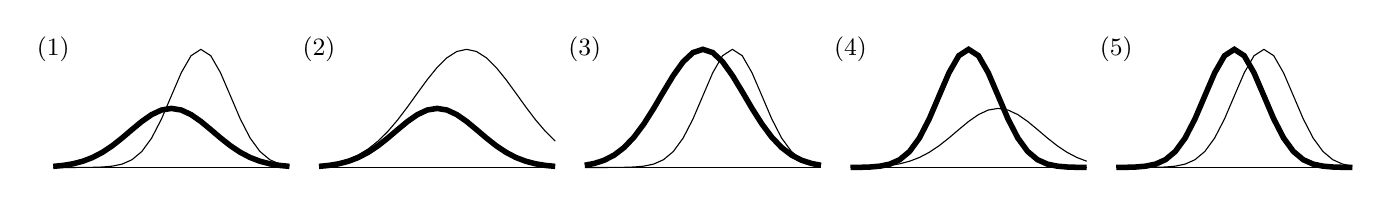
\begin{tikzpicture}[scale=.75]
				\begin{scope}[xshift=0cm,yshift=0cm,domain=-2:2]
				\draw[line width=2pt] plot (\x,{exp(-\x*\x)}) {};
				\draw plot (\x,{2*exp(-(\x-.5)*(\x-.5)/.5)}) {};
				\draw (-2,0) to (2,0);
				\node at (-2,2) {\small (1)};
				\end{scope}
				\begin{scope}[xshift=4.5cm,yshift=0cm,domain=-2:2]
				\draw[line width=2pt] plot (\x,{exp(-\x*\x)}) {};
				\draw plot (\x,{2*exp(-(\x-.5)*(\x-.5)/1.5)}) {};
				\draw (-2,0) to (2,0);
				\node at (-2,2) {\small (2)};
				\end{scope}
				\begin{scope}[xshift=9cm,yshift=0cm,domain=-2:2]
				\draw[line width=2pt] plot (\x,{2*exp(-\x*\x)}) {};
				\draw plot (\x,{2*exp(-(\x-.5)*(\x-.5)/.5)}) {};
				\draw (-2,0) to (2,0);
				\node at (-2,2) {\small (3)};
				\end{scope}
				\begin{scope}[xshift=13.5cm,yshift=0cm,domain=-2:2]
				\draw[line width=2pt] plot (\x,{2*exp(-\x*\x/.5)}) {};
				\draw plot (\x,{1*exp(-(\x-.5)*(\x-.5)/1)}) {};
				\draw (-2,0) to (2,0);
				\node at (-2,2) {\small (4)};
				\end{scope}
				\begin{scope}[xshift=18cm,yshift=0cm,domain=-2:2]
				\draw[line width=2pt] plot (\x,{2*exp(-\x*\x/.5)}) {};
				\draw plot (\x,{2*exp(-(\x-.5)*(\x-.5)/.5)}) {};
				\draw (-2,0) to (2,0);
				\node at (-2,2) {\small (5)};
				\end{scope}
			\end{tikzpicture}
        \end{QBODY}
        \begin{QFROMS}
        \end{QFROMS}
        \begin{QTAGS}\QTAG{B5C1機率與統計}\end{QTAGS}
        \begin{QANS}
            (1)
        \end{QANS}
        \begin{QSOLLIST}
        \end{QSOLLIST}
        \begin{QEMPTYSPACE}
        \end{QEMPTYSPACE}
    \end{QUESTION}
    \begin{QUESTION}
        \begin{ExamInfo}{101}{學測}{單選}{5}
        \end{ExamInfo}
        \begin{ExamAnsRateInfo}{51}{91}{46}{16}
        \end{ExamAnsRateInfo}
        \begin{QBODY}
            若正實數 $x, y$ 滿足 $\log_{10} x =2.8  $, $\log_{10} y = 5.6$,則 $\log_{10} ( x^2 + y)$ 最接近下列哪一個選項的值?
			\begin{QOPS} 
				\QOP   2.8    
				\QOP   5.6 
				\QOP   5.9 
				\QOP   8.4 
				\QOP   11.2 。
			\end{QOPS}
        \end{QBODY}
        \begin{QFROMS}
        \end{QFROMS}
        \begin{QTAGS}\QTAG{B1C3-3對數}\QTAG{B1C3指對數函數}\QTAG{對數律}\end{QTAGS}
        \begin{QANS}
            (3)
        \end{QANS}
        \begin{QSOLLIST}
        \end{QSOLLIST}
        \begin{QEMPTYSPACE}
        \end{QEMPTYSPACE}
    \end{QUESTION}
    \begin{QUESTION}
        \begin{ExamInfo}{101}{學測}{單選}{6}
        \end{ExamInfo}
        \begin{ExamAnsRateInfo}{66}{84}{71}{43}
        \end{ExamAnsRateInfo}
        \begin{QBODY}
            箱中有編號分別為 $0,1, 2, \cdots ,9$   的十顆球。隨機抽取一球,將球放回後,再隨機抽取一球。請問這兩球編號相減的絕對值為下列哪一個選項時,其出現的機率最大?
			\begin{QOPS}
				\QOP  0  
				\QOP  1 
				\QOP  4 
				\QOP  5 
				\QOP  9
			\end{QOPS}
        \end{QBODY}
        \begin{QFROMS}
        \end{QFROMS}
        \begin{QTAGS}\QTAG{B2C3機率}\QTAG{B2C3-2機率的定義與性質}\end{QTAGS}
        \begin{QANS}
            (2)
        \end{QANS}
        \begin{QSOLLIST}
        \end{QSOLLIST}
        \begin{QEMPTYSPACE}
        \end{QEMPTYSPACE}
    \end{QUESTION}
    \begin{QUESTION}
        \begin{ExamInfo}{101}{學測}{單選}{7}
        \end{ExamInfo}
        \begin{ExamAnsRateInfo}{37}{45}{34}{32}
        \end{ExamAnsRateInfo}
        \begin{QBODY}
            空間坐標中有一球面(半徑大於0)與平面 $3x+4y=0$ 相切於原點,請問此球面與三個坐標軸一共有多少個交點? 
			\begin{QOPS} 
				\QOP $1$ 
				\QOP $2$ 
				\QOP $3$ 
				\QOP $4$ 
				\QOP $5$
			\end{QOPS}
        \end{QBODY}
        \begin{QFROMS}
        \end{QFROMS}
        \begin{QTAGS}\QTAG{不是99課綱}\end{QTAGS}
        \begin{QANS}
            (3)
        \end{QANS}
        \begin{QSOLLIST}
        \end{QSOLLIST}
        \begin{QEMPTYSPACE}
        \end{QEMPTYSPACE}
    \end{QUESTION}
\end{QUESTIONS}
\begin{QUESTIONS}
    \begin{QUESTION}
        \begin{ExamInfo}{101}{學測}{多選}{8}
        \end{ExamInfo}
        \begin{ExamAnsRateInfo}{56}{92}{58}{18}
        \end{ExamAnsRateInfo}
        \begin{QBODY}
            設 $f(x) = x^4-5x^3+x^2+ax+b$ 為實係數多項式,且知 $f( i)  =0 $。請問下列哪些選項是多項式方程式 $f (x ) = 0$ 的根?
		\begin{QOPS} 
			\QOP  $-i$ 
			\QOP  $0$
			\QOP  $1$ 
			\QOP  $-5$ 
			\QOP  $5$
		\end{QOPS}
        \end{QBODY}
        \begin{QFROMS}
        \end{QFROMS}
        \begin{QTAGS}\QTAG{B1C2多項式函數}\QTAG{B1C2-3多項式方程式}\QTAG{虛根定理}\end{QTAGS}
        \begin{QANS}
            (1)(2)(5)
        \end{QANS}
        \begin{QSOLLIST}
        \end{QSOLLIST}
        \begin{QEMPTYSPACE}
        \end{QEMPTYSPACE}
    \end{QUESTION}
    \begin{QUESTION}
        \begin{ExamInfo}{101}{學測}{多選}{9}
        \end{ExamInfo}
        \begin{ExamAnsRateInfo}{51}{77}{51}{25}
        \end{ExamAnsRateInfo}
        \begin{QBODY}
            三角形 ABC 是一個邊長為 3 的正三角形,如下圖所示。若在每一邊的兩個三等分點中,各選取一點連成三角形,則下列哪些選項是正確的?

			\begin{QOPS} 
				\QOP 依此方法可能連成的三角形一共有 8 個
				\QOP 這些可能連成的三角形中,恰有 2 個是銳角三角形 \QOP 這些可能連成的三角形中,恰有 3 個是直角三角形
				\QOP 這些可能連成的三角形中,恰有 3 個是鈍角三角形
				\QOP 這些可能連成的三角形中,恰有 1 個是正三角形
			\end{QOPS}
        \end{QBODY}
        \begin{QFROMS}
        \end{QFROMS}
        \begin{QTAGS}\QTAG{乘法原理加法原理}\QTAG{B2C2-1簡單的邏輯與集合}\QTAG{B2C2排列組合}\end{QTAGS}
        \begin{QANS}
            (1)(2)
        \end{QANS}
        \begin{QSOLLIST}
        \end{QSOLLIST}
        \begin{QEMPTYSPACE}
        \end{QEMPTYSPACE}
    \end{QUESTION}
    \begin{QUESTION}
        \begin{ExamInfo}{101}{學測}{多選}{10}
        \end{ExamInfo}
        \begin{ExamAnsRateInfo}{36}{66}{27}{15}
        \end{ExamAnsRateInfo}
        \begin{QBODY}
            設 $O$ 為複數平面上的原點,並令點 $A,B$ 分別代表非零複數 $z,w$。若 $\angle AOB = 90^\circ$,則下列哪些選項必為負實數?
		\begin{QOPS} 
			\QOP $\frac{z}{w}$    
			\QOP $zw$    
			\QOP $(zw)^2$ 
			\QOP $\frac{z^2}{w^2}$ 
			\QOP $(z\overline{w})^2$ (其中 $\overline{w}$ 為 $w$ 的共軛複數)
		\end{QOPS}
        \end{QBODY}
        \begin{QFROMS}
        \end{QFROMS}
        \begin{QTAGS}\QTAG{B5C2三角函數II}\end{QTAGS}
        \begin{QANS}
            (4)(5)
        \end{QANS}
        \begin{QSOLLIST}
        \end{QSOLLIST}
        \begin{QEMPTYSPACE}
        \end{QEMPTYSPACE}
    \end{QUESTION}
    \begin{QUESTION}
        \begin{ExamInfo}{101}{學測}{多選}{11}
        \end{ExamInfo}
        \begin{ExamAnsRateInfo}{37}{62}{29}{20}
        \end{ExamAnsRateInfo}
        \begin{QBODY}
            若實數 $a, b, c,  d$ 使得聯立方程組
			$\left\{\begin{array}{ccc} ax+8y & = & c \\ x-4y & = & 3 \end{array}\right.$
			有解,且聯立方程組 $\left\{\begin{array}{ccc} -3x+by & = & d \\ x-4y & = & 3 \end{array}\right.$
			無解,則下列哪些選項一定正確? 
			\begin{QOPS} 
				\QOP  $a \neq -2$
				\QOP  $c = -6$    
				\QOP  $b =12$    
				\QOP  $d \neq -9$ 
				\QOP  聯立方程組 $\left\{\begin{array}{ccc} ax+8y & = & c \\ -3x+by & = & d \end{array}\right.$無解
			\end{QOPS}
        \end{QBODY}
        \begin{QFROMS}
        \end{QFROMS}
        \begin{QTAGS}\QTAG{B3C3平面向量}\QTAG{B3C3-3面積與二階行列式}\end{QTAGS}
        \begin{QANS}
            (3)(4)
        \end{QANS}
        \begin{QSOLLIST}
        \end{QSOLLIST}
        \begin{QEMPTYSPACE}
        \end{QEMPTYSPACE}
    \end{QUESTION}
    \begin{QUESTION}
        \begin{ExamInfo}{101}{學測}{多選}{12}
        \end{ExamInfo}
        \begin{ExamAnsRateInfo}{42}{64}{40}{22}
        \end{ExamAnsRateInfo}
        \begin{QBODY}
            在坐標平面上,廣義角 $\theta$ 的頂點為原點 $O$,始邊為 $x$ 軸的正向,且滿足 $\tan \theta =\frac{2}{3}$。若 $\theta$ 的終邊上有一點 $P$ ,其 $y$ 坐標為 $-4$ ,則下列哪些選項一定正確? 
			\begin{QOPS} 
				\QOP $P$ 的 $x$ 坐標為 6 
				\QOP $\overline{OP} = 2\sqrt{13}$ 
				\QOP $\cos\theta = \frac{3}{\sqrt{13}}$ 
				\QOP $\sin 2\theta >0$ 
				\QOP $\cos \frac{\theta}{2} <0$。
			\end{QOPS}
        \end{QBODY}
        \begin{QFROMS}
        \end{QFROMS}
        \begin{QTAGS}\QTAG{廣義角}\QTAG{B3C1三角}\QTAG{B3C1-2廣義角與極坐標}\end{QTAGS}
        \begin{QANS}
            (2)(4)
        \end{QANS}
        \begin{QSOLLIST}
        \end{QSOLLIST}
        \begin{QEMPTYSPACE}
        \end{QEMPTYSPACE}
    \end{QUESTION}
    \begin{QUESTION}
        \begin{ExamInfo}{101}{學測}{多選}{13}
        \end{ExamInfo}
        \begin{ExamAnsRateInfo}{45}{79}{40}{16}
        \end{ExamAnsRateInfo}
        \begin{QBODY}
            平面上兩點 $F_1,F_2$ 滿足 $F_1F_2 =4$。設 $d$ 為一實數,令 $\Gamma$ 表示平面上滿足 $|PF_1 -PF_2|=d$ 的所有 $P$ 點所成的圖形,又令 $C$ 為平面上以 $F_1$ 為圓心、 6 為半徑的圓。請問下列哪些選項是正確的?
			\begin{QOPS}
				\QOP 當 $d = 0$ 時,$\Gamma$ 為直線 
				\QOP 當 $d =1$ 時, $\Gamma$ 為雙曲線 
				\QOP 當 $\Gamma = 2$ 時, $\Gamma$ 與圓 $C$ 交於兩點 
				\QOP 當 $d = 4$ 時, $\Gamma$ 與圓 $C$ 交於四點 
				\QOP 當 $d = 8$ 時, $\Gamma$ 不存在。
			\end{QOPS}
        \end{QBODY}
        \begin{QFROMS}
        \end{QFROMS}
        \begin{QTAGS}\QTAG{B4C4-3雙曲線}\QTAG{B4C4二次曲線}\QTAG{圖形}\end{QTAGS}
        \begin{QANS}
            (1)(2)(5)
        \end{QANS}
        \begin{QSOLLIST}
        \end{QSOLLIST}
        \begin{QEMPTYSPACE}
        \end{QEMPTYSPACE}
    \end{QUESTION}
\end{QUESTIONS}
\begin{QUESTIONS}
    \begin{QUESTION}
        \begin{ExamInfo}{101}{學測}{填充}{A}
        \end{ExamInfo}
        \begin{ExamAnsRateInfo}{44}{86}{39}{7}
        \end{ExamAnsRateInfo}
        \begin{QBODY}
            若首項為 $a$,公比為 $0.01$ 的無窮等比級數和等於循環小數 $1.\overline{2}$,則 $a=\TCNBOX{\TCN.\TCN\TCN}$ 。
        \end{QBODY}
        \begin{QFROMS}
        \end{QFROMS}
        \begin{QTAGS}\QTAG{B6C1函數與極限}\end{QTAGS}
        \begin{QANS}
            $1.21$
        \end{QANS}
        \begin{QSOLLIST}
        \end{QSOLLIST}
        \begin{QEMPTYSPACE}
        \end{QEMPTYSPACE}
    \end{QUESTION}
    \begin{QUESTION}
        \begin{ExamInfo}{101}{學測}{填充}{B}
        \end{ExamInfo}
        \begin{ExamAnsRateInfo}{39}{71}{39}{7}
        \end{ExamAnsRateInfo}
        \begin{QBODY}
            設 $A(1,1)$, $B(3,5)$, $C(5,3)$, $D(0,-7)$, $E(2,-3)$ 及 $F(8,-6)$ 為坐標平面上的六個點。若直線 $L$ 分別與三角形 $ABC$ 及三角形 $DEF$ 各恰有一個交點,則 $L$ 的斜率之最小可能值為 $\TCNBOX{\TCN\TCN}$。
        \end{QBODY}
        \begin{QFROMS}
        \end{QFROMS}
        \begin{QTAGS}\QTAG{B3C2-1直線方程式及其圖形}\QTAG{B3C2直線與圓}\end{QTAGS}
        \begin{QANS}
            $-3$
        \end{QANS}
        \begin{QSOLLIST}
        \end{QSOLLIST}
        \begin{QEMPTYSPACE}
        \end{QEMPTYSPACE}
    \end{QUESTION}
    \begin{QUESTION}
        \begin{ExamInfo}{101}{學測}{填充}{C}
        \end{ExamInfo}
        \begin{ExamAnsRateInfo}{56}{90}{65}{13}
        \end{ExamAnsRateInfo}
        \begin{QBODY}
            小明在天文網站上看到以下的資訊「可利用北斗七星斗杓的天璇與天樞這兩顆星來尋找北極星:由天璇起始向天樞的方向延伸便可找到北極星,其中天樞與北極星的距離為天樞與天璇距離的 5 倍。」今小明將所見的星空想像成一個坐標平面,其中天璇的坐標為 (9,8) 及天樞的坐標為 (7,11),依上述資訊可以推得北極星的坐標為 $\TCNBOX{(\TCN\TCN,\TCN\TCN)}$。
        \end{QBODY}
        \begin{QFROMS}
        \end{QFROMS}
        \begin{QTAGS}\QTAG{線性組合}\QTAG{B3C3-1平面向量的表示法}\QTAG{B3C3平面向量}\end{QTAGS}
        \begin{QANS}
            $(-3,26)$
        \end{QANS}
        \begin{QSOLLIST}
        \end{QSOLLIST}
        \begin{QEMPTYSPACE}
        \end{QEMPTYSPACE}
    \end{QUESTION}
    \begin{QUESTION}
        \begin{ExamInfo}{101}{學測}{填充}{D}
        \end{ExamInfo}
        \begin{ExamAnsRateInfo}{37}{83}{27}{1}
        \end{ExamAnsRateInfo}
        \begin{QBODY}
            設點 $A(-2,2)$、$B(4,8)$ 為坐標平面上兩點,且點 $C$ 在二次函數 $y = \frac{1}{2}x^2$ 的圖形上變動。當 $C$ 點的 $x$ 坐標為 $\TCNBOX{\TCN\TCN}$ 時,內積 $\lvec{AB}\cdot \lvec{AC}$ 有最小值 $\TCNBOX{\TCN\TCN}$ 。
        \end{QBODY}
        \begin{QFROMS}
        \end{QFROMS}
        \begin{QTAGS}\QTAG{B3C3-2平面向量的內積}\QTAG{B3C3平面向量}\end{QTAGS}
        \begin{QANS}
            $-1,-3$
        \end{QANS}
        \begin{QSOLLIST}
        \end{QSOLLIST}
        \begin{QEMPTYSPACE}
        \end{QEMPTYSPACE}
    \end{QUESTION}
    \begin{QUESTION}
        \begin{ExamInfo}{101}{學測}{填充}{E}
        \end{ExamInfo}
        \begin{ExamAnsRateInfo}{46}{85}{39}{14}
        \end{ExamAnsRateInfo}
        \begin{QBODY}
            在邊長為13的正三角形 $ABC$ 上各邊分別取一點 $P,Q,R$,使得 $APQR$ 形成一平行四邊形,如右圖所示:若平行四邊形 $APQR$ 的面積為 $20\sqrt{3}$,則線段 PR 的長度為 $\TCNBOX{\TCN}$ 。
			
			\begin{tikzpicture}[scale=.15]
				\begin{scope}\small
						\foreach \n/\i/\j/\l in{B/0/0/240,C/0/13/300,Q/0/8/300,A/60/13/90,P/60/8/120}{
								\node[inner sep=0pt,draw,circle] (v\n)at (\i:\j) [label=\l:$\n$] {};
						}
						\node[inner sep=0pt,draw,circle]  (vR) at ($(0:13)!.38!(60:13)$) [label=30:$R$] {};
						\foreach \i/\j in{B/C,C/A,A/B,P/Q,Q/R}
								\draw (v\i) to (v\j);
						\draw[dotted] (vP) to (vR);
				\end{scope}
			\end{tikzpicture}
        \end{QBODY}
        \begin{QFROMS}
        \end{QFROMS}
        \begin{QTAGS}\QTAG{面積}\QTAG{B3C1-3正弦定理與餘弦定理}\QTAG{B3C1三角}\end{QTAGS}
        \begin{QANS}
            $7$
        \end{QANS}
        \begin{QSOLLIST}
        \end{QSOLLIST}
        \begin{QEMPTYSPACE}
        \end{QEMPTYSPACE}
    \end{QUESTION}
    \begin{QUESTION}
        \begin{ExamInfo}{101}{學測}{填充}{F}
        \end{ExamInfo}
        \begin{ExamAnsRateInfo}{40}{80}{37}{3}
        \end{ExamAnsRateInfo}
        \begin{QBODY}
            設 $m,n$ 為正實數,橢圓 $\frac{x^2}{m}  + \frac{y^2}{n} =1$ 的焦點分別為 $F_1 (0,2)$ 與 $F_2 (0,-2)$。若此橢圓上有一點 $P$ 使得 $\triangle PF_1 F_2$ 為一正三角形,則 $m=\TCNBOX{\TCN\TCN} , n = \TCNBOX{\TCN\TCN}$。
        \end{QBODY}
        \begin{QFROMS}
        \end{QFROMS}
        \begin{QTAGS}\QTAG{B4C4二次曲線}\QTAG{B4C4-2橢圓}\end{QTAGS}
        \begin{QANS}
            $12, 16$
        \end{QANS}
        \begin{QSOLLIST}
        \end{QSOLLIST}
        \begin{QEMPTYSPACE}
        \end{QEMPTYSPACE}
    \end{QUESTION}
    \begin{QUESTION}
        \begin{ExamInfo}{101}{學測}{填充}{G}
        \end{ExamInfo}
        \begin{ExamAnsRateInfo}{23}{54}{13}{2}
        \end{ExamAnsRateInfo}
        \begin{QBODY}
            坐標空間中,在六個平面 $x=\frac{14}{13}$,  $x=\frac{1}{13}$ , $y=1$,  $y=-1$, $z=-1$ 及 $z=-4$ 所圍成的長方體上隨機選取兩個相異頂點。若每個頂點被選取的機率相同,則選到兩個頂點的距離大於 3 之機率為 $\TCNBOX{\FR{\TCN}{\TCN}}$ 。
        \end{QBODY}
        \begin{QFROMS}
        \end{QFROMS}
        \begin{QTAGS}\QTAG{B4C2空間中的平面與直線}\QTAG{B4C2-1平面方程式}\QTAG{B2C3機率}\QTAG{B2C3-2機率的定義與性質}\QTAG{距離}\end{QTAGS}
        \begin{QANS}
            $\FR{3}{7}$
        \end{QANS}
        \begin{QSOLLIST}
        \end{QSOLLIST}
        \begin{QEMPTYSPACE}
        \end{QEMPTYSPACE}
    \end{QUESTION}
\end{QUESTIONS}
